%----------------------------------------------------------------------------------------
\chapter{Introduzione}
\label{chap:introduzione}
%----------------------------------------------------------------------------------------


\section{Contesto}
\label{sec:contesto}

Le attuali tendenze tecnologiche, in particolare la rapida espansione dell'\ac{IoT}, stanno favorendo una crescente integrazione dei dispositivi computazionali nell'ambiente circostante, aprendo nuove prospettive per servizi e applicazioni innovative.
%
Tra gli esempi più rilevanti si annoverano sistemi di monitoraggio ambientale, reti di sensori intelligenti, infrastrutture urbane connesse e robotica collaborativa.

I paradigmi di programmazione tradizionali, che individuano l'unità programmabile nel singolo dispositivo, risultano ormai inadatti allo sviluppo di applicazioni distribuite su larga scala.
%
Questa prospettiva individuale evidenzia le complessità legate alla gestione della comunicazione, della sincronizzazione e del coordinamento tra nodi, che diventano parti integranti del codice applicativo del sistema distribuito.
%
Con l'aumentare della complessità, tali sistemi manifestano limiti di design, come scarsa modularità e riusabilità, difficoltà nel deployment e nel testing.
%
Di conseguenza, la progettazione di sistemi distribuiti viene spesso percepita come una sfida ardua e rischiosa, generando timore e resistenza invece che stimolare la valorizzazione delle potenzialità offerte da un ecosistema di dispositivi cooperanti.



\subsection{Aggregate Programming}
\label{sec:programmazioneaggregata}

\ac{AP} \cite{AC} è un paradigma di macroprogrammazione \cite{macroprogramming} ideato per lo sviluppo di Sistemi Collettivi Adattivi (CAS). 
%
A differenza degli approcci tradizionali, in cui il comportamento globale di un sistema emerge dall’interazione dei comportamenti locali dei singoli dispositivi (logica bottom-up), \ac{AP} adotta una prospettiva globale (top-down): il comportamento desiderato dell’intera rete viene specificato attraverso un unico programma aggregato, in cui l’unità programmabile non è più il singolo dispositivo, bensì l’intero collettivo.
%
Saranno poi il linguaggio e gli strumenti sottostanti a derivare automaticamente i comportamenti locali necessari affinché il sistema si auto-organizzi per soddisfare le specifiche globali.

Dal punto di vista formale, \ac{AP} si fonda su \ac{FC} \cite{AC} (\Cref{sec:fieldcalculus}), un linguaggio minimale progettato per specificare il comportamento aggregato di un sistema distribuito. L'astrazione centrale è quella del \textit{campo computazionale} \cite{AC} (\Cref{campo}): una mappa, potenzialmente dinamica, che associa a ciascun dispositivo della rete un valore. Da una prospettiva globale, un programma aggregato implementa una serie di trasformazioni su queste strutture dati distribuite. L'approccio a campi consente di creare algoritmi distribuiti riusabili tramite funzioni componibili — da campo a campo — organizzabili in librerie di complessità crescente per costruire interi servizi applicativi.
\paragraph{Proprietà}

I sistemi sviluppati con \ac{AP} possiedono intrinsecamente proprietà di adattabilità e resilienza, che si manifestano in risposta a variazioni dell'ambiente operativo, come cambiamenti nella topologia della rete, guasti dei dispositivi o fluttuazioni delle risorse disponibili. 
%
Inoltre, tali sistemi sono in grado di gestire efficientemente un numero crescente di dispositivi, mantenendo basso l’overhead comunicativo e l’efficienza computazionale.

\paragraph{Architettura a livelli}
\ac{AP} semplifica la complessità della coordinazione distribuita grazie a una struttura a più livelli di astrazione (\Cref{fig:ac-architecture}), costruita a partire da \ac{FC} \cite{AC}.

La scelta di basarsi su un calcolo minimale e matematico permette di dimostrare formalmente le proprietà dei costrutti fondamentali e di definire operatori generali con caratteristiche verificabili. Questi operatori possono essere utilizzati per realizzare librerie di alto livello, preservando nelle composizioni le proprietà dimostrate a livello dei singoli componenti.
\begin{figure}
    \centering
    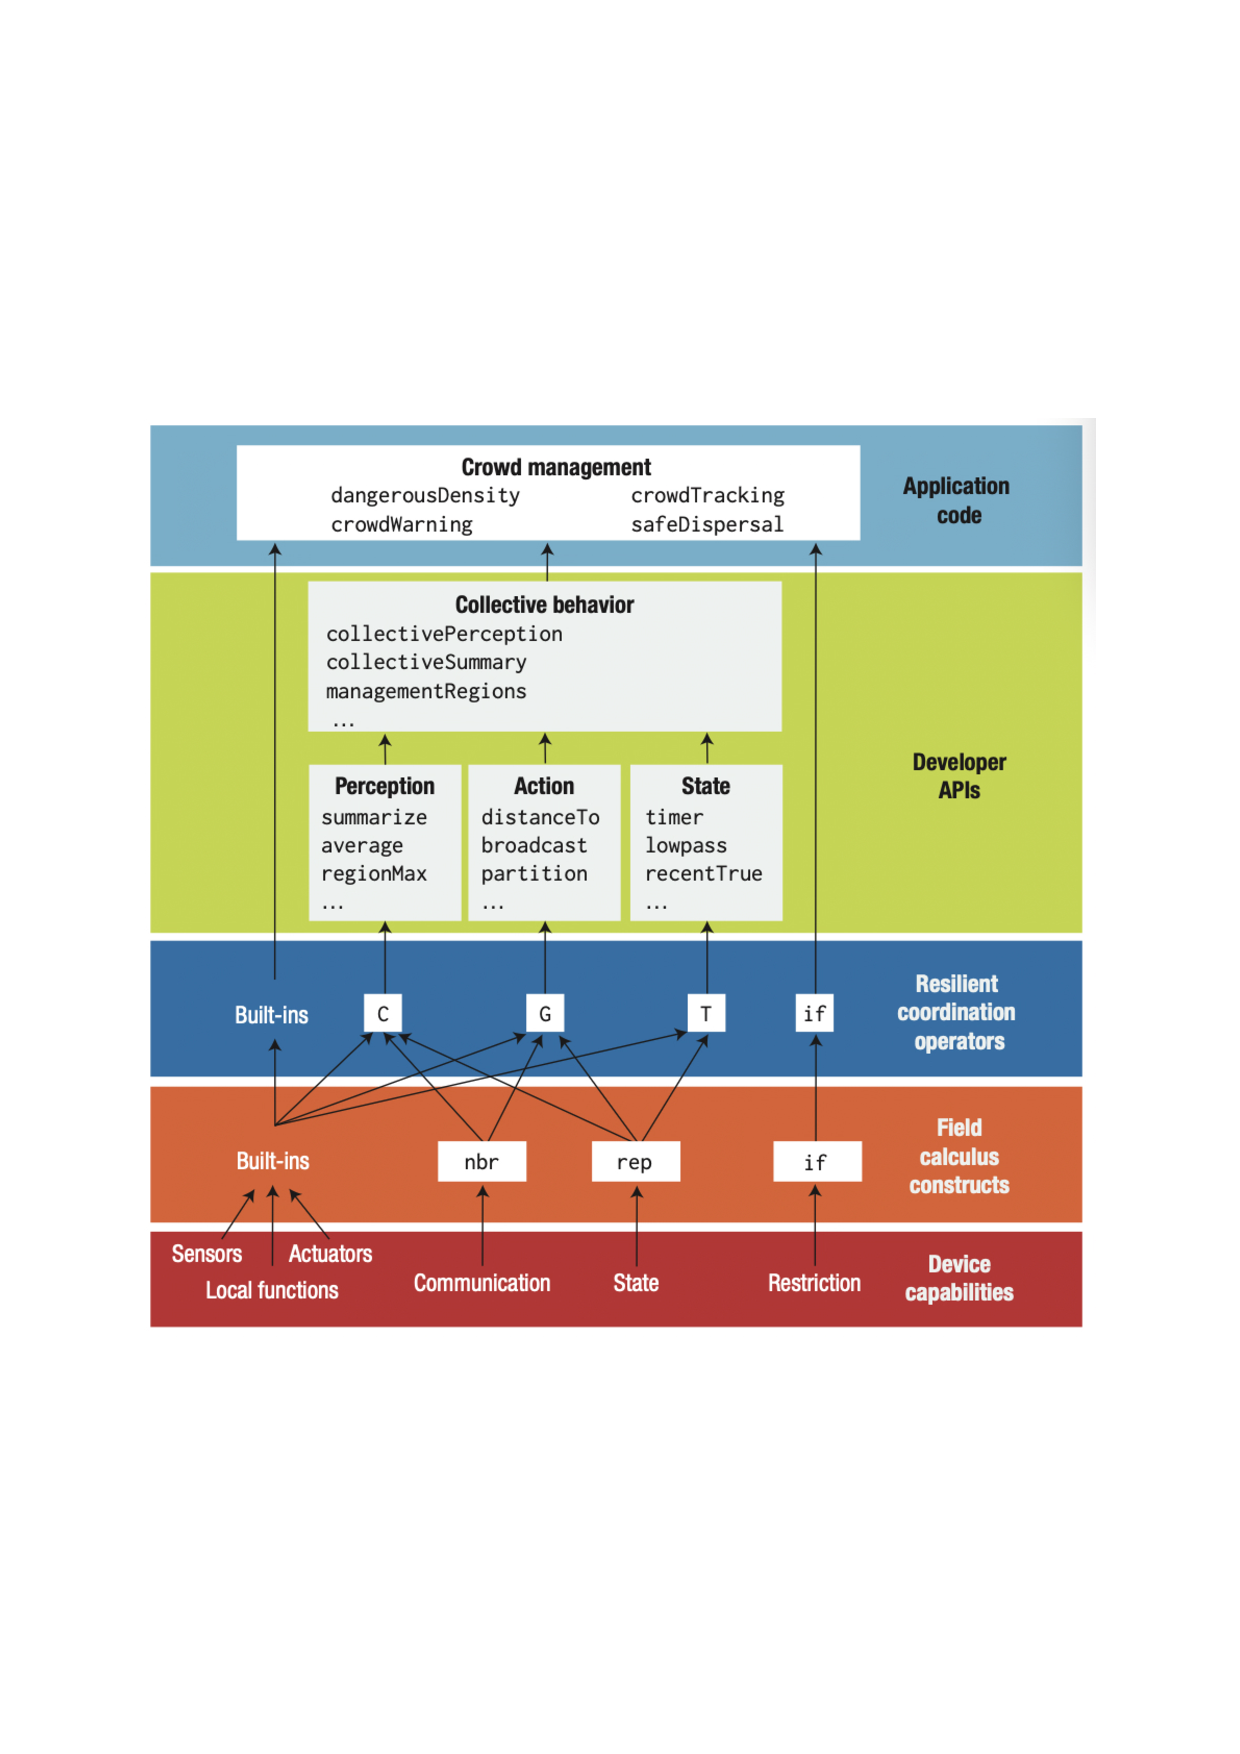
\includegraphics[width=.8\linewidth]{figures/ac-architecture.pdf}
    \caption{
        Architettura a livelli della programmazione aggregata \cite{AC}.
        Le capacità del dispositivo sono sfruttate per implementare i costrutti di \ac{FC}, che a loro volta costituiscono la base per la creazione di un limitato numero di operatori aggregati di cui si può provare la resilienza. Tali costrutti sono così generali da poter essere utilizzati per costruire librerie di alto livello per la programmazione aggregata.}
    \label{fig:ac-architecture}
\end{figure}


\subsection{Field Calculus e Higher-Order Field Calculus}
\label{sec:fieldcalculus}

\ac{FC} è un linguaggio funzionale minimale, progettato per offrire i costrutti fondamentali necessari alla manipolazione dei campi \cite{HFC}. In questo formalismo, l'astrazione unificante è quella del \textit{campo computazionale}, attorno al quale si organizzano i costrutti del linguaggio che permettono di operare su tali strutture.

\paragraph{Campo computazionale \label{campo}} Un campo computazionale è una struttura dati distribuita nello spazio e nel tempo che associa ad ogni dispositivo un valore.
%
A titolo esemplificativo, si consideri una rete di sensori di temperatura distribuiti su un'area geografica: tale configurazione può essere interpretata come un campo computazionale discreto, in cui ogni sensore rappresenta un punto del campo e il valore a esso associato corrisponde alla temperatura rilevata in quel istante.

\paragraph{Modello di Esecuzione} Una computazione può essere osservata da due prospettive diverse: locale e globale \cite{HFC}.

Dal punto di vista aggregato (globale), è possibile specificare il comportamento collettivo del sistema attraverso una serie di trasformazioni su campi computazionali.
%
Ad esempio, l’input di una computazione può essere un campo di temperature, in cui a ciascun dispositivo viene associato il valore rilevato dal proprio sensore; l’output, invece, può essere un campo booleano che indica quali dispositivi superano una determinata soglia di temperatura.

Dal punto di vista locale, la computazione è vista dal singolo dispositivo \(\delta_i\), che esegue periodicamente un programma \texttt{P} in round di esecuzione asincroni.
%
In questa visione, il dispositivo \(\delta_i\) non può percepire l'intero campo globale, ma solo una proiezione limitata ai dispositivi entro il proprio raggio di comunicazione, definita come \textit{campo di vicinato}, ovvero una mappa \(\phi: \delta \to v\) che associa a ciascun vicino \(\delta_j\) il valore \(v_j\) più recente.
%
In ogni round, il dispositivo: 
\begin{enumerate*}[label=\roman*), itemjoin={{; }}, itemjoin*={{; }}]
    \item raccoglie i valori dal proprio campo di vicinato \(\phi_i\)
    \item ottiene le informazioni dall'ambiente (tramite sensori)
    \item recupera lo stato interno
    \item valuta il programma \texttt{P} utilizzando queste informazioni
    \item aggiorna il proprio stato e invia il valore risultante ai vicini
    \item attende il successivo round di esecuzione
\end{enumerate*} \cite{HFC}.

\paragraph{Sintassi}

I costrutti fondamentali di \ac{FC} \cite{AC} sono:
\begin{itemize}
    \item Chiamate a funzione: \texttt{b(\(e_1, \dots, e_n\))} applica la funzione \texttt{b} agli argomenti \texttt{\(e_1, \dots, e_n\)}, restituendo un nuovo campo computazionale.

    \item Dinamica Temporale: $\texttt{rep(\(e_0\)) \{(x) => e\}}$ è fondamentale per modellare l'evoluzione nel tempo di un campo. Inizializza una variabile di stato locale $\texttt{x}$ con il valore iniziale $\texttt{e}_0$ e, ad ogni round di esecuzione, aggiorna $\texttt{x}$ con il risultato dell'espressione $\texttt{e}$. L'espressione $\texttt{e}$ può fare riferimento al valore precedente di $\texttt{x}$, consentendo la definizione di processi iterativi.

    \item Interazione Spaziale: $\texttt{nbr\{e\}}$ modella l'evoluzione spaziale del campo, consentendo a un dispositivo di accedere ai valori calcolati dai vicini nell'ultimo round di esecuzione. Restituisce un campo di vicinato ($\phi$) che mappa l'identificatore di ogni vicino all'espressione $\texttt{e}$ valutata in quel dispositivo. I campi di vicinato così ottenuti possono essere manipolati tramite funzioni di aggregazione spaziale, come $\texttt{min-hood}$, $\texttt{max-hood}$, $\texttt{sum-hood}$ e altre.

    \item Restrizione del dominio: \texttt{if (\(e_0\)) \{\(e_1\)\} else \{\(e_2\)\}} partiziona la rete in due sottoinsiemi \(D_{true}\) e \(D_{false}\) in base alla valutazione di \texttt{\(e_0\)}. Se un dispositivo \(\delta\) appartiene a \(D_{true}\), valuta esclusivamente l’espressione \(e_1\), ignorando \(e_2\); viceversa, se appartiene a \(D_{false}\), valuta solo \(e_2\). In entrambi i casi, le informazioni di stato e i valori scambiati con i vicini non vengono condivisi tra i due rami: quando un dispositivo passa da un ramo all’altro, le variabili di stato vengono reinizializzate e i valori precedenti vengono persi. Se è necessario condividere informazioni tra i rami, si può utilizzare il costrutto \texttt{mux(\(e_0, e_1, e_2\))}, che valuta entrambe le espressioni \texttt{\(e_1\)} ed \texttt{\(e_2\)}, prima del partizionamento, restituendo il valore corrispondente a \texttt{\(e_0\)}.

    \item Share: la combinazione dei costrutti \texttt{rep} e \texttt{nbr} permette di modellare l'evoluzione sia spaziale che temporale di un campo. Tuttavia, come evidenziato in \cite{UniversalityFC}, la loro integrazione introduce un ritardo implicito nel sistema che può causare la perdita di round. Per risolvere questo problema, l'approccio presentato in \cite{Share} introduce il costrutto \texttt{share}:
    \[
    \texttt{share(\(e_1\)) \{(x) => \(e_2\)\}}
    \]
    Nonostante la sintassi sia identica a quella di \texttt{rep}, i due si distinguono radicalmente per l'interpretazione della variabile \texttt{x} ad ogni round. Nel caso di \texttt{share}, \texttt{x} non rappresenta un valore locale (come in \texttt{rep}), bensì un campo di vicinato ($\phi$) che contiene i valori condivisi dai vicini nel round precedente. L'espressione \texttt{\(e_2\)} ha quindi il compito di elaborare questo campo di vicinato per produrre un nuovo valore locale, che sarà poi utilizzato come \texttt{\(e_1\)} nel round successivo e condiviso con i vicini.
\end{itemize}

\paragraph{Allineamento} Ogni nodo deve comunicare esclusivamente con i dispositivi che si trovano nello stesso contesto di esecuzione, ossia che hanno seguito lo stesso percorso di valutazione del programma: hanno invocato le stesse funzioni e preso le stesse decisioni. Tali dispositivi si definiscono \textit{allineati}.

Si consideri l'esempio in \cref{lst:alignment}, in cui sono definite due funzioni, \texttt{f1} e \texttt{f2}, entrambe contenenti il costrutto \texttt{nbr} applicato alla stessa espressione \texttt{e1}. Quando un dispositivo esegue \texttt{nbr \{e1\}} all'interno di \texttt{f1}, deve recuperare esclusivamente i valori dei vicini che hanno valutato l'espressione nel medesimo contesto. Di conseguenza, i valori prodotti dai vicini per \texttt{nbr \{e1\}} all'interno di \texttt{f2} risultano irrilevanti.
\lstinputlisting[
    language=Scala,
    label={lst:alignment},
    caption={Allineamento tra le esecuzioni di \texttt{nbr} in contesti diversi}
]{listings/alignment.scala}

Questo aspetto risulta particolarmente evidente nel costrutto \texttt{if}, che non si limita a determinare quale ramo eseguire, bensì suddivide il dominio in due gruppi distinti, ciascuno con il proprio contesto di esecuzione. In questi casi, l'allineamento diventa fondamentale per garantire che la comunicazione avvenga solo tra nodi che hanno scelto lo stesso ramo.

Poiché non esiste una memoria condivisa per tracciare lo stato computazionale, è necessario introdurre meccanismi di allineamento capaci di monitorare ogni nodo e determinare quali risultino effettivamente allineati. In un linguaggio di programmazione ideale, questi dettagli di basso livello dovrebbero rimanere trasparenti all'utente finale.

\paragraph{Higher-Order Field Calculus} \ac{FC} è stato esteso in \cite{HFC} con l'introduzione di \ac{HFC}, che consente di trattare le funzioni come valori. Questa estensione abilita capacità fondamentali quali: 
\begin{enumerate*}[label=\roman*), itemjoin={{; }}, itemjoin*={{; }}]
    \item accettare funzioni come argomenti e restituirle come risultati
    \item creare funzioni dinamicamente
    \item trasferirle tra dispositivi (tramite \texttt{nbr}) e memorizzarle o modificarle nel tempo (tramite \texttt{rep})
\end{enumerate*}.

\subsection{XC}
\label{sec:xc}

\ac{XC} è un calcolo formale che definisce una semantica operazionale per la programmazione aggregata, generalizzando ed estendendo le capacità di \ac{FC} \cite{XC}. È progettato per supportare lo sviluppo di comportamenti collettivi adattivi astraendo la gestione di aspetti di basso livello quali concorrenza, esecuzione asincrona, comunicazione e gestione dei guasti.

\paragraph{Modello di Esecuzione}
Ogni dispositivo, indicato con \(\delta_i\), comunica con i propri vicini tramite uno scambio di messaggi. Il funzionamento dei nodi si articola in round di esecuzione asincroni. In ogni round, ciascun dispositivo esegue un programma \ac{XC}, elabora i messaggi ricevuti e produce nuovi messaggi da inviare al vicinato (\Cref{fig:xc-rounds}).

Data la natura asincrona del sistema, può verificarsi che un dispositivo completi più round prima che un vicino ne termini uno. In questi casi, il vicino considererà solo l'ultimo messaggio ricevuto, sovrascrivendo i precedenti.\begin{figure}
    \centering
    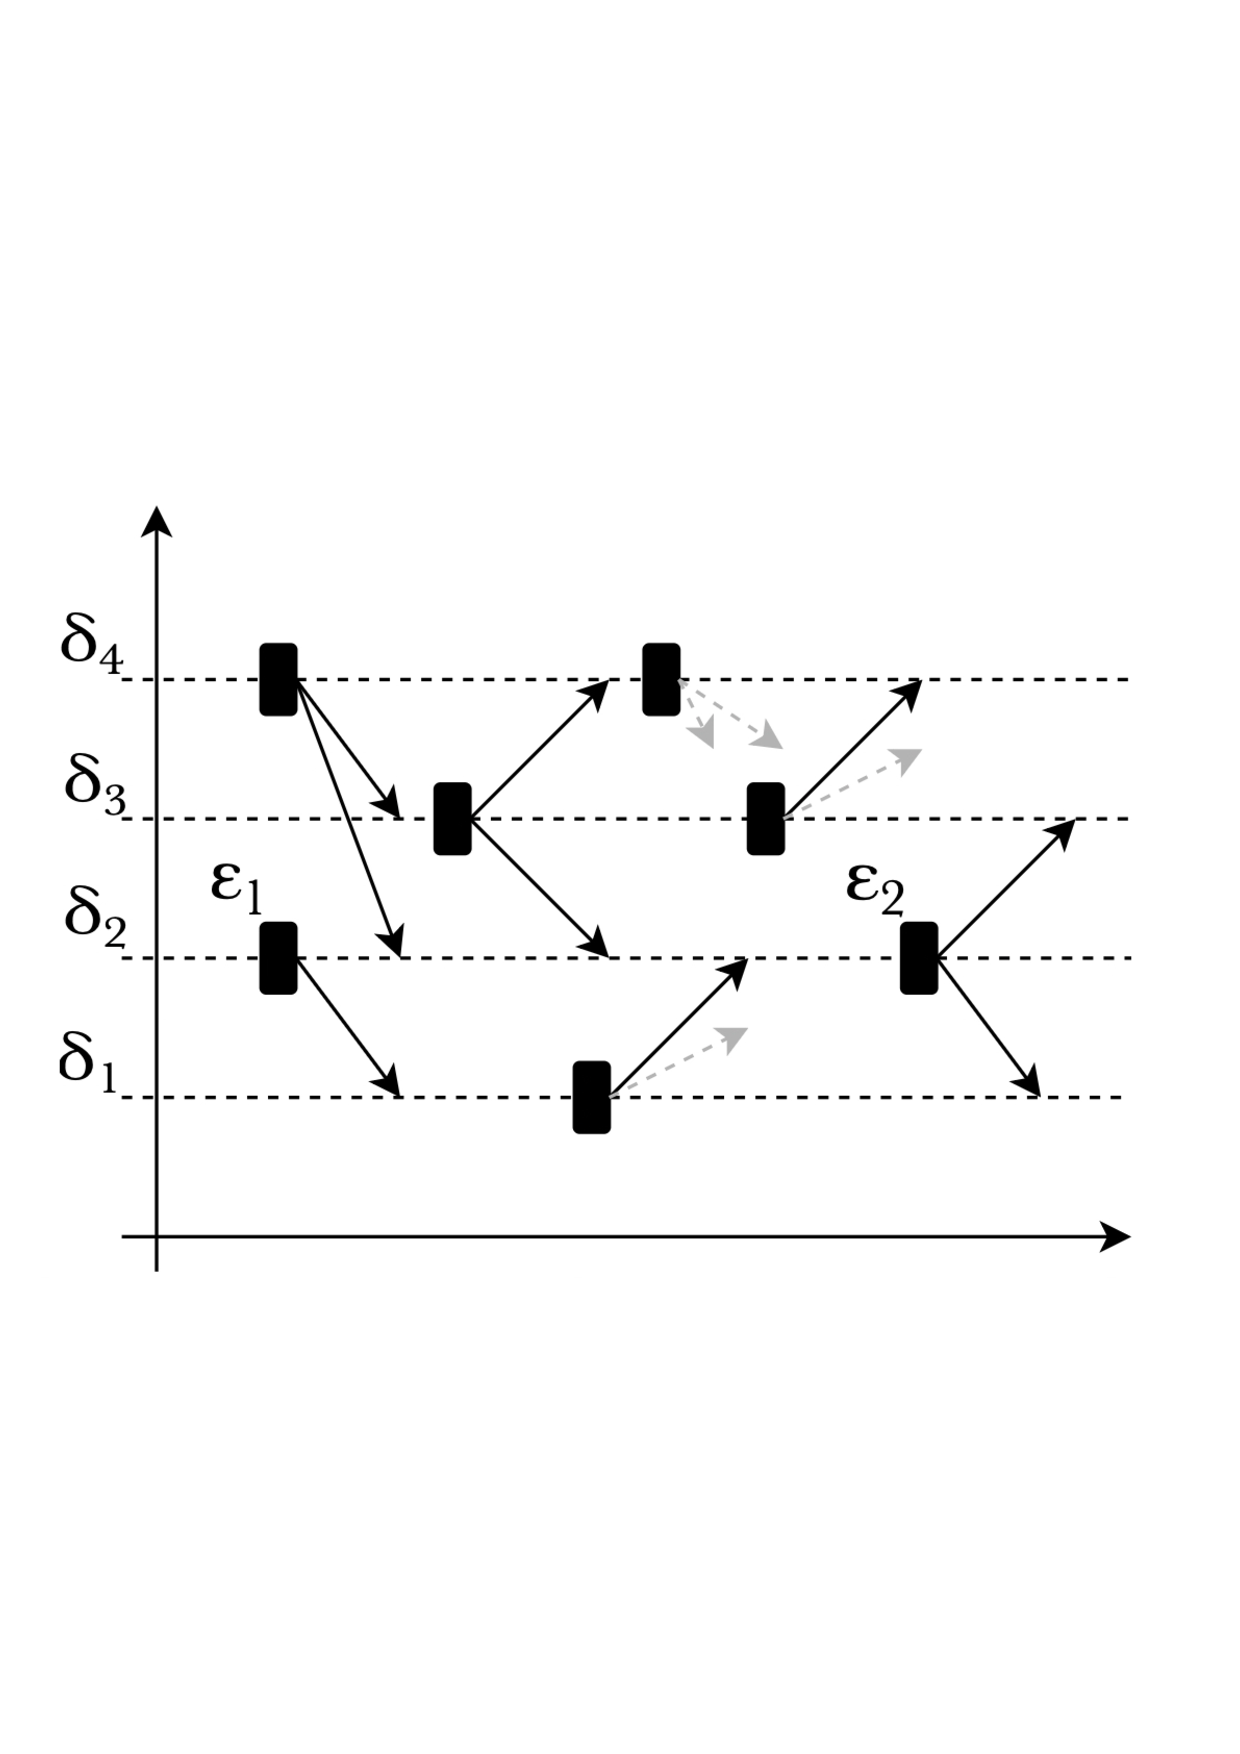
\includegraphics[width=.8\linewidth]{figures/xc-rounds.pdf}
    \caption{Modello di esecuzione di \ac{XC}: il dispositivo \(\delta_i\) esegue il programma \ac{XC} nei round \(\varepsilon_n\) e invia i messaggi ai vicini al termine di ciascuno \cite{XC}.}
    \label{fig:xc-rounds}
\end{figure}

\paragraph{Tipi di dato} Nel formalismo \ac{FC}, si distinguono due categorie di valori: i valori locali \(\ell\) e i campi di vicinato \(\phi\). Quest'ultimi sono mappe che associano un valore locale a ciascun identificatore di dispositivo e vengono impiegati per rappresentare i messaggi ricevuti dai vicini. Tuttavia, \ac{FC} impone che solo i valori locali \(\ell\) possano essere inviati. Ciò implica che ogni nodo trasmetta necessariamente lo stesso messaggio a tutti i suoi vicini (comunicazione \textit{isotropica}), limitando l'espressività del linguaggio impedendo l'invio di messaggi differenziati.

\ac{XC} risolve questa limitazione unificando le due categorie in una singola classe di valori denominata \texttt{nvalues} (\(v\)), consentendo a ciascun dispositivo di inviare messaggi diversi a vicini differenti (comunicazione \textit{anisotropica}).

Un \texttt{nvalue} è una struttura dati che associa un valore locale \(\ell_i\) a ciascun identificatore di dispositivo \(\delta_i\) specificato e include un valore di default \(\ell\):

\[v = \ell[\delta_1 \to \ell_1, \dots, \delta_n \to \ell_n]\]

Tale notazione significa che \(v\) assume il valore di default \(\ell\) per tutti i dispositivi, ad eccezione di quelli esplicitamente specificati (\(\delta_1, \dots, \delta_n\)), ai quali sono associati i valori \(\ell_1, \dots, \ell_n\). Un valore locale \(\ell\) può essere automaticamente convertito in un \texttt{nvalue} con \(\ell\) come valore di default e senza eccezioni (\(\ell[]\)).

Questa unificazione semplifica notevolmente il sistema di tipi rispetto a \ac{FC} e, grazie alla flessibilità degli \texttt{nvalues}, \ac{XC} risulta più espressivo e versatile nella gestione della comunicazione eterogenea tra dispositivi.

\paragraph{exchange} La comunicazione in \ac{XC} è costruita attorno ad un'unica primitiva chiamata \texttt{exchange} \cite{XC}, che incapsula in unico costrutto computazione, comunicazione e gestione dello stato.

La sintassi è la seguente:
%
\[
\texttt{exchange(\(e_i\), (n)) => return \(e_r\) send \(e_s\)}
\]
%
Dove:
\begin{itemize}
    \item \(\mathbf{e_i}\): È l'espressione che determina il valore locale iniziale. Tale valore funge da default per l'$\texttt{nvalue}$ dei messaggi nel primo round o quando non sono ancora stati ricevuti messaggi dai vicini.
    \item \(\mathbf{n}\): È una variabile che, ad ogni round di esecuzione, viene automaticamente sostituita con l'\texttt{nvalue} che incapsula i messaggi ricevuti dai vicini.
    \item \(\mathbf{e_r}\): È l'espressione che definisce il valore locale di ritorno del costrutto, che rappresenta il risultato del round corrente del dispositivo.
    \item \(\mathbf{e_s}\): È l'espressione che definisce l'\texttt{nvalue} dei messaggi che il dispositivo invierà ai vicini al termine del round corrente.
\end{itemize}

Ogni costrutto di \ac{FC} può essere espresso in termini di \texttt{exchange}, come illustrato in \cite{XC}. Il fatto che ogni programma \ac{FC} possa essere codificato in \ac{XC}, permette a quest'ultimo di ereditare tutte le proprietà di resilienza e universalità dimostrate per \ac{FC} \cite{UniversalityFC}.

\newpage
\section{Motivazione}
\label{sec:motivazione}

Il panorama della programmazione aggregata è caratterizzato da diversi linguaggi e framework che implementano i concetti fondamentali di \ac{FC}, ognuno con specifici vantaggi e svantaggi. 
Tra le soluzioni più note e consolidate si annoverano MIT Proto \cite{proto} (\Cref{sec:mitproto}), Protelis \cite{protelis} (\Cref{sec:protelis}), ScaFi \cite{scafi} (\Cref{sec:scafi}) e FCPP \cite{fcpp} (\Cref{sec:fcpp}). 

In questo scenario, l'ultima proposta è Collektive (\Cref{sec:collektive}), un \ac{DSL} sviluppato in Kotlin. Collektive si pone l'obiettivo di sintetizzare i punti di forza dei linguaggi esistenti, superandone al contempo le limitazioni strutturali, rappresentando così un passo in avanti nel contesto della programmazione aggregata.


\subsection{MIT Proto}
\label{sec:mitproto}

\emph{Proto} \cite{proto}, riconosciuto come il precursore della programmazione aggregata, fu concepito originariamente da Jonathan Bachrach e Jacob Beal e si basa su \emph{Amorphous Computing} \cite{Amorphous}. 

È un linguaggio puramente funzionale, con una sintassi ispirata a Lisp (\Cref{lst:mitprotoexample}).
\lstinputlisting[
    language=Lisp,
    label={lst:mitprotoexample},
    caption={Dimostrazione della sintassi di Proto}
]{listings/proto/gradient.proto}

A supporto delle sue funzionalità, veniva fornito un simulatore integrato che consentiva di eseguire e testare i programmi in ambienti simulati. Successivamente fu sviluppato anche WebProto, un ambiente di prototipazione web che permetteva di scrivere e testare codice aggregato direttamente dal browser.

Lo sviluppo del linguaggio è stato interrotto nel 2016 e Proto è stato ufficialmente dismesso in favore di Protelis \cite{protelis} (\Cref{sec:protelis}), che ne ha raccolto l'eredità concettuale e operativa.

La sintassi e i costrutti del linguaggio verranno esaminati in dettaglio nel \cref{chap:mitproto}.

\subsection{Protelis}
\label{sec:protelis}

\emph{Protelis} \cite{protelis} è un linguaggio di programmazione funzionale che implementa i concetti di \ac{HFC} (\Cref{sec:fieldcalculus}). La sua sintassi è ispirata al linguaggio $\text{C}$, il che lo rende più accessibile rispetto al suo predecessore. È inoltre caratterizzato dall'essere debolmente tipizzato (\Cref{lst:protelisexample}).

Protelis è un linguaggio stand-alone per la \ac{JVM}, sviluppato utilizzando Xtext, un framework specializzato nella creazione di \ac{DSL}.
%
L'esecuzione dei programmi avviene tramite un interprete che valuta periodicamente il codice aggregato. Questo gestisce in modo automatico la comunicazione tra dispositivi e l'interazione con l'ambiente. Poiché l'interprete è stato scritto da zero, i meccanismi di basso livello, come l'allineamento, sono gestiti in modo trasparente per l'utente finale, senza richiedere interventi espliciti nel codice applicativo.
%
L'integrazione con la JVM garantisce portabilità tra sistemi e dispositivi, oltre a facilitare l'importazione di numerose librerie e API tramite i meccanismi di reflection di Java. Tuttavia, la necessità di una JVM rappresenta una limitazione per l'impiego in ambienti con risorse estremamente ristrette, come quelli tipici dell'\ac{IoT}, riducendo l'eterogeneità dei dispositivi utilizzabili.

Attualmente il linguaggio è attivamente mantenuto, ma lo sviluppo di nuove funzionalità è stato congelato.

\lstinputlisting[
    language=Java,
    label={lst:protelisexample},
    caption={Dimostrazione della sintassi di Protelis}
]{listings/protelis/distanceTo}

\subsection{ScaFi}
\label{sec:scafi}

\emph{ScaFi} \cite{scafi} (Scala Fields) è un framework per la programmazione aggregata, realizzato come \ac{DSL} interno al linguaggio Scala e basato su \ac{FC} (\ref{sec:fieldcalculus}), in particolare sulla variante FScaFi \cite{fscafi}.

Offre un ecosistema completo per lo sviluppo di programmi aggregati, comprendente librerie, strumenti di simulazione e la possibilità di prototipazione rapida via browser grazie a ScaFi Web \cite{scafiweb}.

L’integrazione come \ac{DSL} interno consente a ScaFi di beneficiare direttamente della sintassi (\Cref{lst:scafiexample}), del compilatore e degli strumenti di Scala, risultando così più semplice da mantenere, immediatamente familiare per chi già conosce il linguaggio ospite e in grado di sfruttare appieno il potente sistema di tipi di Scala.

Questa scelta, tuttavia, comporta anche alcune limitazioni: la sintassi è vincolata ai costrutti validi di Scala e, aspetto cruciale per la programmazione aggregata, possono emergere involontariamente dettagli di basso livello che non dovrebbero essere esposti all’utente, come la gestione dell’allineamento. Inoltre, essendo pensato principalmente per l’esecuzione sulla JVM, ScaFi condivide le stesse limitazioni di applicabilità già riscontrate per Protelis (\ref{sec:protelis}).

\lstinputlisting[
    language=Scala,
    label={lst:scafiexample},
    caption={Dimostrazione della sintassi di ScaFi}
]{listings/scafi/distanceTo.scala}

\subsection{FCPP}
\label{sec:fcpp}

\emph{FCPP} \cite{fcpp} rappresenta la prima implementazione nativa di \ac{AP} in \(\text{C++}\).

L'utilizzo di \(\text{C++}\) come linguaggio di base è un elemento chiave, poiché consente l'esecuzione diretta del codice sui dispositivi, senza la necessità di una macchina virtuale. Questo approccio offre due vantaggi principali: da un lato, risulta particolarmente adatto a dispositivi con risorse limitate, come sistemi di microcontrollori e dispositivi embedded tipici dell'\ac{IoT}, superando così le restrizioni imposte dalla dipendenza dalla JVM che caratterizzano soluzioni come Protelis e ScaFi; dall'altro, permette di ottenere prestazioni elevate nell'implementazione del paradigma aggregato.

Tuttavia, la scelta di \(\text{C++}\) comporta anche alcune criticità. La complessità della sintassi (\Cref{lst:fcppexample}) e la limitata ergonomia rispetto ad altre soluzioni rendono difficile l’adozione da parte di un ampio pubblico di sviluppatori. Inoltre, la gestione dell’allineamento non è trasparente, ma richiede interventi manuali tramite macro. Sebbene FCPP sia pensato come una piattaforma flessibile ed estensibile, il numero di funzionalità attualmente disponibili risulta inferiore rispetto alle alternative.

\lstinputlisting[
    language=C++,
    label={lst:fcppexample},
    caption={Dimostrazione della sintassi di FCPP}
]{listings/fcpp/distance-to.cpp}



\subsection{Collektive}
\label{sec:collektive}

\emph{Collektive}\footnote{\url{https://github.com/Collektive}} nasce dall'esigenza di disporre di un linguaggio che 
\begin{enumerate*}[label=\roman*), itemjoin={{; }}, itemjoin*={{; }}]
    \item garantisca una gestione dell'allineamento robusta e completamente trasparente
    \item sia multipiattaforma e quindi adatto a operare su reti di dispositivi eterogenei
    \item offra una sintassi moderna, espressiva ed ergonomica
    \item possa contare su un ecosistema maturo e ricco di funzionalità grazie al linguaggio host
\end{enumerate*}.

I linguaggi analizzati in precedenza non riescono a soddisfare tutti questi requisiti contemporaneamente: Protelis offre una buona gestione dell'allineamento ma dipende dalla JVM; ScaFi è anch'esso vincolato alla JVM e presenta un allineamento debole; FCPP è nativo e performante ma manca di ergonomia, semplicità d'uso e trasparenza.

Analogamente a ScaFi, Collektive è un \ac{DSL} interno; tuttavia, si basa su Kotlin, la cui natura multi-piattaforma, resa possibile dal progetto \ac{KMP}\footnote{\url{https://kotlinlang.org/docs/multiplatform.html}}, consente l’operatività su reti di dispositivi eterogenei, che spaziano da server con elevate capacità di calcolo (tramite JVM), a dispositivi mobili (Android e iOS), offrendo inoltre la possibilità di eseguire nativamente applicazioni su piattaforme quali Windows, MacOS e Linux, sia su architetture x86 che ARM.

A differenza di ScaFi, il compilatore di Kotlin è stato esteso tramite un apposito plugin per gestire automaticamente l'allineamento del codice aggregato.

Se si volesse gestire manualmente l'allineamento, sarebbe sufficiente adottare un semplice \ac{DSL}; tuttavia, il codice risulterebbe esposto a meccanismi di basso livello, rendendo la scrittura dei programmi aggregati più complessa e soggetta ad errori (\Cref{lst:ckmanuallyaligned}).

\lstinputlisting[
    language=Kotlin,
    label={lst:ckmanuallyaligned},
    caption={Come apparirebbe un programma aggregato in Collektive se l'allineamento fosse gestito manualmente dallo sviluppatore invece che automaticamente dal compilatore.}
]{listings/collektive/GradientManuallyAligned.kt}

Il plugin del compilatore si occupa di iniettare automaticamente il codice necessario per gestire l’allineamento e la proiezione dei campi di vicinato, permettendo agli sviluppatori di scrivere programmi aggregati in Kotlin in modo naturale.

\lstinputlisting[
    language=Kotlin,
    label={lst:ckexample},
    caption={Dimostrazione della sintassi di Collektive: il compilatore si occupa automaticamente di gestire l'allineamento per conto dello sviluppatore.}
]{listings/collektive/GradientAutomaticallyAligned.kt}





\newpage
\section{Obiettivo}
\label{sec:obiettivo}

Quando emerge un nuovo linguaggio o framework, è fondamentale che gli sviluppatori possano sfruttare le conoscenze acquisite con le tecnologie precedenti. I sistemi moderni, quindi, devono offrire una guida chiara su come realizzare soluzioni già presenti. Senza questa guida e senza esempi pratici, l'adozione di nuove tecnologie può essere rallentata dalla curva di apprendimento e dalla scarsa familiarità.

Fornire esempi concreti di trasposizione di sistemi legacy a nuove soluzioni dimostra l'espressività del nuovo sistema rispetto ai precedenti, riduce significativamente il tempo di apprendimento e accresce la fiducia nella nuova tecnologia.

Questo lavoro si propone di trasporre una serie di esempi di programmazione aggregata (\Cref{chap:trasposizione}) realizzati originariamente in Proto (\Cref{chap:mitproto}) al linguaggio Collektive (\Cref{chap:collektive}).
